\documentclass{article}
% pre\'ambulo

\usepackage{lmodern}
\usepackage[T1]{fontenc}
\usepackage[spanish,activeacute]{babel}
\usepackage{mathtools}
\usepackage{graphicx}
\usepackage{listings}
\usepackage{tabu}
\usepackage{hyperref}
\usepackage[utf8]{inputenc}
\usepackage{multicol}
\usepackage{amsmath}
\usepackage{amssymb}
\usepackage{enumerate}
\usepackage{amsthm}
\usepackage{wrapfig}
\usepackage{esvect}
\usepackage{subcaption}
\usepackage{wasysym}
\usepackage{yhmath}
\usepackage{adjustbox}

\spanishdecimal{.}




% Default fixed font does not support bold face
\DeclareFixedFont{\ttb}{T1}{txtt}{bx}{n}{8} % for bold
\DeclareFixedFont{\ttm}{T1}{txtt}{m}{n}{8}  % for normal

% Custom colors
\usepackage[usenames,dvipsnames]{color}
\definecolor{deepblue}{rgb}{0,0,0.5}
\definecolor{deepred}{rgb}{0.6,0,0}
\definecolor{deepgreen}{rgb}{0,0.5,0}

% Python style for highlighting
\newcommand\pythonstyle{\lstset{
language=Python,
basicstyle=\ttm,
otherkeywords={self},             % Add keywords here
keywordstyle=\ttb\color{deepblue},
emph={MyClass,__init__},          % Custom highlighting
emphstyle=\ttb\color{deepred},    % Custom highlighting style
stringstyle=\color{deepgreen},
frame=tb,                         % Any extra options here
showstringspaces=false            % 
}}


% Python environment
\lstnewenvironment{python}[1][]
{
\pythonstyle
\lstset{#1}
}
{}

% Python for external files
\newcommand\pythonexternal[2][]{{
\pythonstyle
\lstinputlisting[#1]{#2}}}

% Python for inline
\newcommand\pythoninline[1]{{\pythonstyle\lstinline!#1!}}

\usepackage{amsmath} % or simply amstext
\newcommand{\angstrom}{\text{\normalfont\AA}}
\newcommand*{\everymodeprime}{\ensuremath{\prime}}

\title{Tarea 1}
\author{Francisco Felipe Carrasco Varela}

\usepackage{vmargin}

\setpapersize{A4}
\setmargins{1.82cm}       % margen izquierdo
{1.3cm}                        % margen superior
{17.5cm}                      % anchura del texto
{23.42cm}                    % altura del texto
{10pt}                           % altura de los encabezados
{1cm}                           % espacio entre el texto y los encabezados
{0pt}                             % altura del pie de página
{2cm}                           % espacio entre el texto y el pie de página

\usepackage{array,booktabs,tabularx,caption, ragged2e}
\newcolumntype{C}{>{\centering\arraybackslash}X}

\begin{document}
\begin{minipage}{2.3cm}

\includegraphics[width=2cm]{../logo_byn.png}
\vspace{0.5cm}
\end{minipage}
\begin{minipage}{\linewidth}
\textsc{\raggedright \footnotesize
Pontificia Universidad Católica de Chile \\
Facultad de Física -- Instituto de Astrof'isica \\
Astronom'ia -- AST0111 \\
Primer Semestre 2020}
\end{minipage}
\begin{center}
{\LARGE \textbf{Ayudant'ia 3 -- Soluci'on}}

\vspace{3mm}

Profesora: Viviana Guzm'an

Ayudantes: Camila Aravena Gonz'alez (\texttt{cfaravena1$@$uc.cl}) -- Francisco Carrasco Varela (\texttt{ffcarrasco$@$uc.cl})

\end{center}
\begin{center}
\noindent\rule{12cm}{0.4pt}
\end{center}

Esta ayudant'ia tratar'a principalmente de repasar conceptos.

\vspace{3mm}

\textbf{Problema 1. D'ia sideral y d'ia solar}

\begin{enumerate} [a)]
\item ?`Cu'al es la diferencia entre el a'no tr'opico y el a'no sideral?

\emph{Soluci'on:}

El a'no sideral (o a'no sid'ereo) es el tiempo que transcurre entre dos pasos consecutivos de la Tierra por un mismo punto de su 'orbita. ?`C'omo se sabe cuando se alcanza este ``mismo punto de su 'orbita''? Porque, para ello, se toman como referencia las estrellas (especialmente las lejanas que, como vimos, dada su lejan'ia var'ian muy poco o pr'acticamente nada por paralaje). Tiene una duraci'on de, aproximadamente, 365.25 d'ias solares medios (d'ias que duran 24 horas).

\begin{figure}[!h]
  \centering
  \begin{minipage}[b]{0.4\textwidth}
    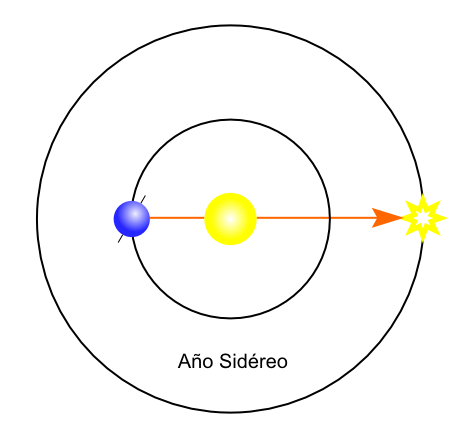
\includegraphics[width=\textwidth]{ano_sideral.png}
    %\caption*{Flower one.}
  \end{minipage}
  \hfill
  \begin{minipage}[b]{0.4\textwidth}
    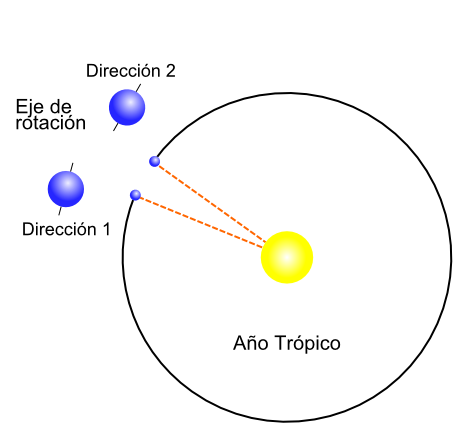
\includegraphics[width=\textwidth]{ano_tropico.png}
    %\caption*{Flower two.}
  \end{minipage}
  \caption{Ilustraciones para el a'no sideral (izquierda) y a'no tr'opico (derecha). La imagen del a'no sideral muestra la posici'on de la Tierra respecto a una estrella de campo.} \label{anos}
\end{figure}

Por otro lado, el a'no tr'opico (o a'no solar) es el tiempo que demora la Tierra en llegar a la misma posici'on en el ciclo de las estaciones, vistas desde la Tierra. Por ejemplo: el tiempo que transcurre entre un equinoccio vernal a otro equinoccio vernal, o el tiempo que pasa entre un solsticio de invierno a otro solsticio de invierno. Es, aproximadamente, unos  $\sim20$ minutos m'as corto que el a'no sideral. Por lo que tiene una duraci'on de aproximadamente 365.24 d'ias solares medios. 
Recordemos que el Sol alcanza su m'axima/m'inima altura sobre el cielo (m'axima/m'inima declinaci'on posible) en los solsticios y est'a alineado con el ecuador celeste en los equinoccios. Por lo que, por ejemplo, un a'no tr'opico podr'iamos medirlo empezando a contar los d'ias desde que el Sol dej'o de estar en su punto m'as alto en el cielo y vuelva a estar en ese punto m'as alto. Como dato extra, la Luna y otros planetas pueden interactuar gravitacionalmente con la Tierra, variando casi imperceptiblemente el valor del a'no tr'opico (en unos pocos minutos o segundos), por lo mismo se cre'o el a'no tropical medio.

Notar entonces que los a'nos siderales son levemente mayores a los a'nos tr'opicos en duraci'on. Una diferencia esquem'atica de esto puede ser apreciada en la Figura \ref{anos}.

\item ?`A qu'e se debe esta diferencia?

\emph{Soluci'on:}

Esta diferencia se debe gracias a, principalmente, la precesi'on de la Tierra. Recordemos que hablamos de  equinoccio o solsticio a los puntos donde el eje de rotaci'on de la Tierra se al'inea  (en los solsticios) o es perpendicular (equinocios) a la l'inea imaginaria que hay entre el Sol y la Tierra. Si no recuerda del todo qu'e/c'omo son los equinoccios/solsticios observe la Figure \ref{ec_celeste}. Ya que la Tierra sufre de su precesi'on, estos puntos se ven levemente corridos y la direcci'on del eje de rotaci'on cambia muuuuy levemente. Lo que hace esto, como se puede ver en la Figura \ref{anos} (derecha), es que se alcanzan los equinoccios/solsticios levemente antes comparados a la posici'on en la 'orbita casi un a'no atr'as. Es decir, en la Figura \ref{anos} (derecha), para una persona que est'a primero ubicado donde dice ``Direcci'on 1'' ver'a, por ejemplo, un equinoccio. Casi un a'no despu'es la Tierra har'a su movimiento de precesi'on y, gracias a este, la persona lograr'a ver nuevamente ese equinoccio en la posici'on donde dice ``Direcci'on 2'', pero esta vez en una posici'on de la 'orbita un poco antes comparado al a'no anterior. 

\begin{figure}[!ht]
\begin{center}
\begin{tabular}{ll}
  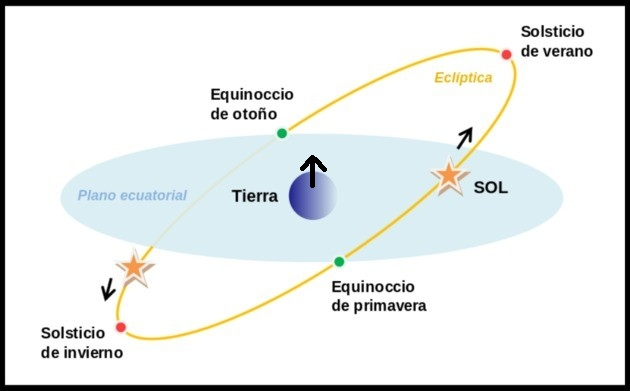
\includegraphics[width=0.5\textwidth]{ec_celeste_2.jpg} 
\end{tabular}
\caption{{\small Equinoccios y solsticios. Notar que los nombres de los equinoccios y solsticios est'an en funci'on del hemisferio Norte. Es decir, por ejemplo, donde en la figura diga ``equinoccio de primavera'' para nosotros, en nuestro hemisferio, ser'a ``equinoccio de oto'no''. La flecha negra al centro muestra el eje de rotaci'on de la Tierra.}}\label{ec_celeste}
\end{center} 
\end{figure}

\item ?`En cu'al de los dos a'nos se basa nuestro calendario? ?`Sideral o tr'opico?
\end{enumerate}

\begin{wrapfigure}{l}{5.5cm}
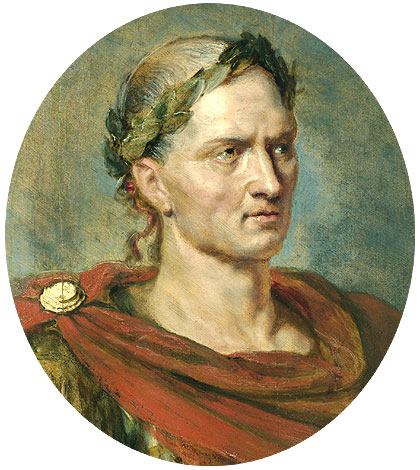
\includegraphics[width=4.8cm]{julio_cesar.jpg}
\caption{Recreaci'on del emperador Julio Cesar.}\label{julio_cesar}
\end{wrapfigure} 

Para dar un breve resumen hist'orico, desde el a'no 46 A.C. hasta el año 1582 D.C. se utiliz'o lo que se conoc'ia como el calendario juliano, el cual fue instaurado y expandido por el Imperio Romano. Su nombre est'a dedicado a Julio C'esar (100 A.C - 44. A.C.) y fue una de las muchas reformas impartidas por 'el al imperio romano, incluso luego de su muerte. Este calendario asum'ia que los d'ias duraban 365.25 d'ias (es decir, a'no sideral).

Luego de eso, en el a'no 1582 D.C., el papa Gregorio XIII implement'o el calendario actualmente usado por casi todos los pa'ises del mundo: el calendario gregoriano. Este calendario ten'ia la intenci'on de ``fijar'' ciertas fechas religiosas. Habían ciertos momentos astrales (como los equinoccios) que indicaban ciertos ritos religiosos. Se fij'o que la Pascua ser'ia celebrada el siguiente Domingo luego de la luna llena despu'es del equinoccio de primavera. Es decir, se esperaba el equinoccio de primavera (en el hemisferio Norte), se esperaba una luna llena y, luego, el Domingo siguiente se celebraba la Pascua (recordar que la religi'on en aquella 'epoca ten'ia much'isimo peso). En el a'no 325 D.C. el equinoccio de primavera (en el hemisferio Norte) era el 21 de Marzo, pero a medida que el tiempo pasaba el equinoccio iba sucediendo cada vez m'as temprano. Hasta el punto en que en el a'no 1582 el desfase ya era de 10 d'ias. 


\begin{wrapfigure}{r}{5.5cm}
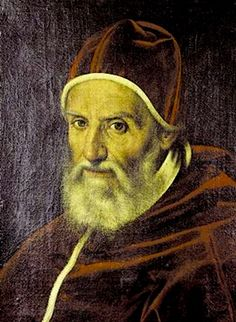
\includegraphics[width=4.8cm]{gregorio_xiii.jpg}
\caption{Retrato del Papa Gregorio XIII.}\label{gregorio_xiii}
\end{wrapfigure} 

Lo que encontraron ciertos investigadores de aquella 'epoca es que el tiempo que ocurre entre dos equinoccios vernales (equinoccio de oto'no en nuestro hemisferio) no eran 365.25 d'ias, sino 365.24 d'ias. B'asicamente, lo que encontraron es que el a'no tr'opico medido por ellos duraba $\sim 11$ minutos m'as que el a'no sideral, valor que luego fue mejor ajustado/medido.
El papa Gregorio XIII form'o un comit'e con los astr'onomos de la 'epoca --conocida como la ``Comisi'on del Calendario''-- y decidieron hacer una especie de ``traspaso'' del calendario juliano al gregoriano. Lo que concluyeron fue que, ya que acababan de encontrar que cada a'no hab'ian 11 minutos ``extras'', 'estos ya hab'ian sido contados desde que fue creado el calendario juliano. Por lo que para corregir esto decidieron que el traspaso del calendario juliano al gregoriano ser'ia el siguiente: el 4 de Octubre de 1582 (juliano) pasar'ia a ser el 14 de Octubre de 1582 (gregoriano). Es decir, por m'as loco que suene, de una d'ia a otro el calendario pas'o del 4 de Octubre al 14 de Octubre\footnote{De hecho, si buscan calendarios hist'oricos, ver'an que muchos de estos llegan hasta el a'no 1583. Porque antes de eso el calendario gregoriano, que usamos hoy en d'ia, no exist'ia.}. Y es el que se ha usado hasta el d'ia de hoy.

Por lo tanto, respondiendo a la pregunta principal, lo que se utiliza a d'ia de hoy en nuestro calendario ``civil'' del d'ia a d'ia es el a'no tr'opico. Pero los astr'onomos como somos medios especiales nos interesan m'as la posici'on de los astros (m'as que la de los equinoccios, que no deja de ser algo que a'un as'i consideramos), por lo mismo el calendario que se utiliza en astronom'ia es el juliano. Y, por lo mismo, m'as adelante en la carrera ver'an que las fechas donde fueron tomadas ciertos datos est'an basadas en el calendario juliano con d'ias julianos.
\vspace{5mm}

\textbf{Problema 2. Analema.} La Figura \ref{Analema} muestra un analema. 

\begin{enumerate} [a)]

\item ?`Qu'e es un analema?

\emph{Soluci'on:}

Si nos ponemos en un lugar fijo todos los d'ias y tomamos una foto a la misma hora al mismo trozo del cielo todos los d'ias encontrar'iamos algo similar a la Figura \ref{analema_casa} o \ref{Analema}. Es decir, un analema es una especie de diagrama que el Sol va dibujando a lo largo del a'no gracias al cambio de posici'on aparente en el cielo.

\begin{figure}[!ht]
\begin{center}
\begin{tabular}{ll}
  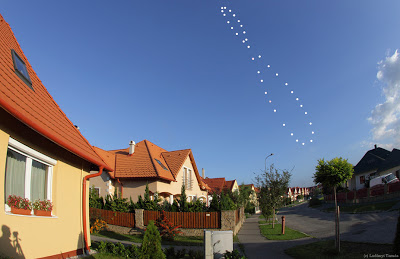
\includegraphics[width=0.5\textwidth]{analema_casa.jpg} 
\end{tabular}
\caption{{\small Analema medido desde una residencia com'un y corriente.}}\label{analema_casa}
\end{center} 
\end{figure}

\newpage

\item ?`Qu'e informaci'on podemos obtener de un analema si es que, adem'as, conocemos el hemisferio en el cual nos encontramos?

\emph{Soluci'on:}

A pesar de que los analemas no son m'as que la inclinaci'on del eje de rotaci'on de la Tierra, respecto al plano del Sol, la excentricidad del planeta y otras cosas; podemos hacer la inversa: conocer las caracter'isticas de dónde nos encontramos conociendo la forma del analema. O, por ejemplo, reconocer que si el Sol est'a en cierta posici'on del analema entonces estamos en cierta 'epoca del a'no (equinoccios o solsticios) sin necesidad de un calendario. Alguna informaci'on de lo que se puede encontrar de un analema puede ser visto en la Figura \ref{analema_informacion}.

\begin{figure}[!ht]
\begin{center}
\begin{tabular}{ll}
  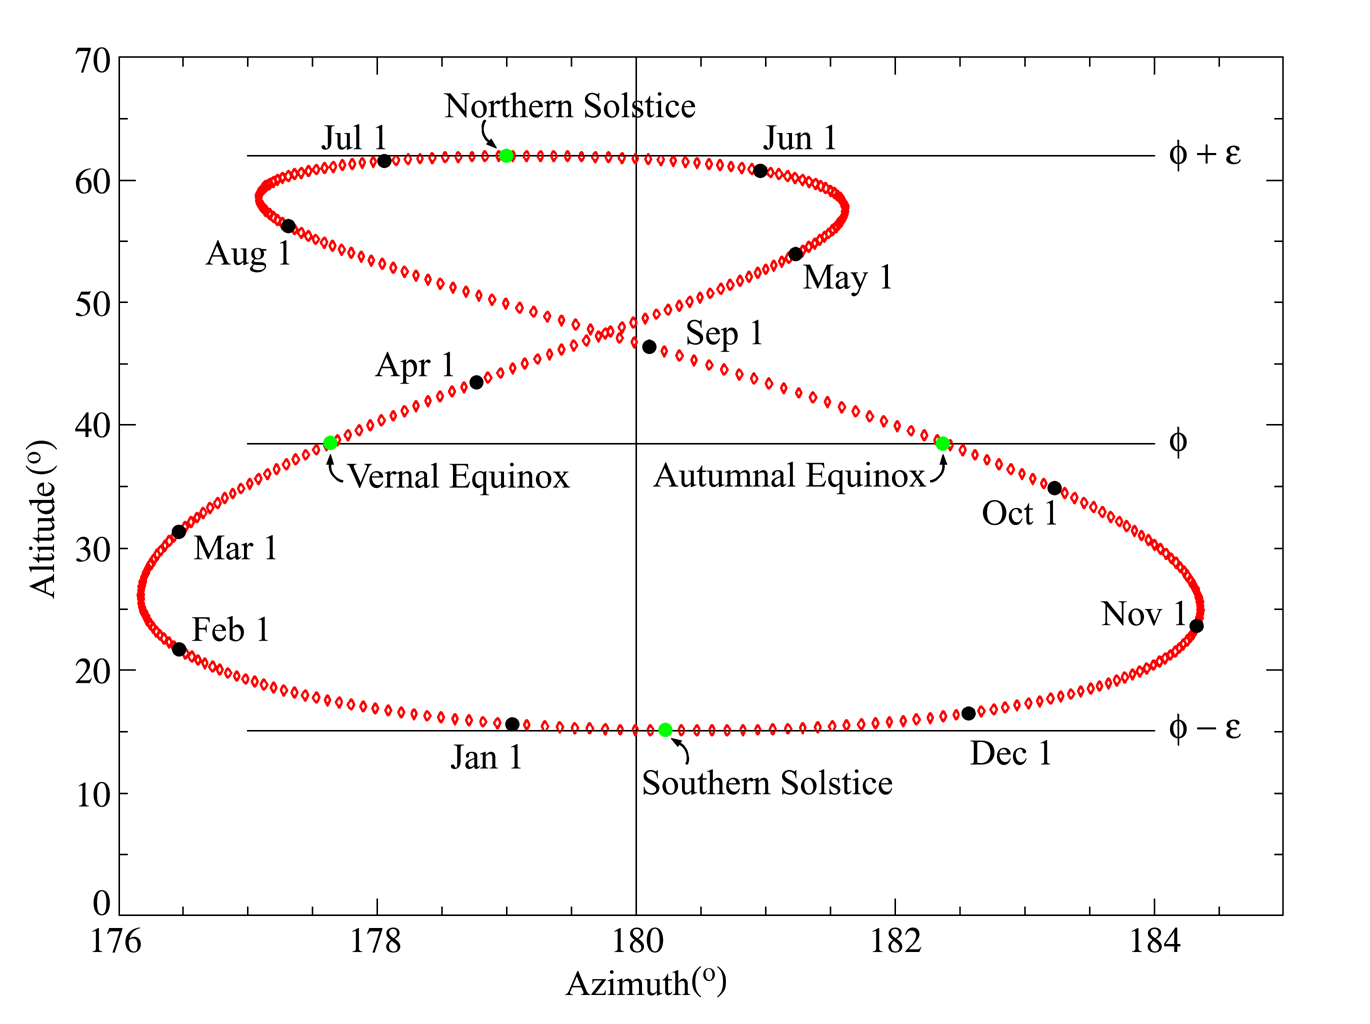
\includegraphics[width=0.7\textwidth]{analemma_information.png} 
\end{tabular}
\caption{{\small Altura y azimut ('angulo que se mide, tomando el Norte como el grado 0, hacia el este) para un analema. Dependiendo de la posici'on del Sol en el analema podemos extraer cierta informaci'on de 'este como, por ejemplo, si se encuentra en alg'un equinoccio o solsticio. En este caso, $\phi$ est'a definido como $\phi = 90^\circ - \text{latitud}$. Y $\varepsilon$ es la inclinaci'on del eje de rotaci'on con respecto al plano del Sol. En el caso de la Tierra $\varepsilon = 23.5^\circ$. Este analema fue construido en el Royal Observatory (latitud $+51.47^\circ$, longitud $0^\circ$), por lo que $\phi \approx 38.52^\circ$ --misma altura a donde ocurrir'an los equinnocios, pero distintos azimuts--, el solsticio de invierno ocurrir'a a una altura de aproximadamente $\phi - \varepsilon \approx 15.02^\circ$ y el solsticio de verano a una altura de $\phi+\varepsilon \approx 62.02^\circ$.}}\label{analema_informacion}
\end{center} 
\end{figure}

Si desea jugar por su cuenta, en \url{https://alokm.com/astro/analemmagenerator.html#} puede ver c'omo se ven los analemas en distintos planetas del Sistema Solar. O c'omo var'ia 'este a medida que cambia cosas como, la excentricidad con la que se orbita alrededor del Sol entre otros par'ametros. Por lo que podr'ia ver c'omo se ve un analema no s'olo desde otro planeta, sino tambi'en desde alg'un otro objeto como un cometa.

\newpage

\item Dibuje en la Figura \ref{Analema} en qu'e punto del analema el Sol se encuentra en el Solsticio de Verano, Invierno o los Equinoccios. Para ello asume que el Sur se encuentra en la parte inferior del dibujo.
\end{enumerate}

\emph{Soluci'on:}

En el hemisferio Norte la parte m'as ancha del ``8'' que se forma est'a en la parte inferior. Al cambiar de hemisferio, la parte m'as ancha se encuentra en la parte superior. La gente en el Polo Norte s'olo ver'a la parte superior del analema de la Figura \ref{Analema}, mientras que la gente en el Polo Sur s'olo puede ver la parte inferior de la Figura \ref{Analema}.

\begin{figure}[!ht]
\begin{center}
\begin{tabular}{ll}
  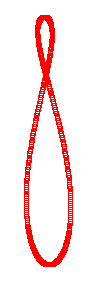
\includegraphics[width=0.1\textwidth]{Analema.png}
\end{tabular}
\caption{Analema en alg'un lugar del hemisferio norte. Recuerde que en esta figura el Sur se encuentra en la parte inferior (o apuntando hacia abajo).}\label{Analema}
\end{center} 
\end{figure}

La Figura  \ref{Analema} puede ser interpretada, \emph{desde el hemisferio Sur} (con los respectivos equinoccios y solsticios desde 'este) en la Figura \ref{Analema_explained}:

\begin{figure}[!ht]
\begin{center}
\begin{tabular}{ll}
  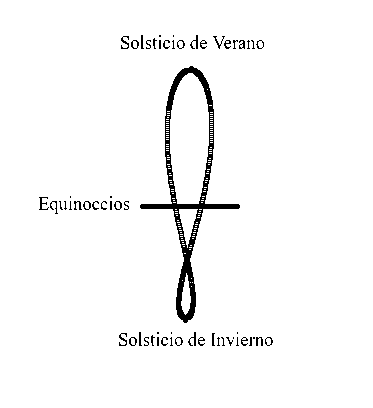
\includegraphics[width=0.5\textwidth]{Analema_explained.png}
\end{tabular}
\caption{Analema en alg'un lugar del hemisferio sur. Los equinoccios y solsticios tambi'en est'an en funci'on del hemisferio sur.}\label{Analema_explained}
\end{center} 
\end{figure}


\newpage

\textbf{Problema 3.} Suponga que usted observa todos los d'ias alg'un astro apenas este sale del horizonte. Si usted lo observ'o hoy, usted debe estimar a qu'e hora saldr'a mañana. 

?`Por qu'e este objeto va saliendo antes (o despu'es) del horizonte? Para ello le puede ser de utilidad realizar un dibujo.

\emph{Soluci'on:}

Asumiendo que la Tierra da una vuelta cada 365, aproximadamente, podemos decir que la Tierra recorre $\frac{360^{\circ}}{365 \ \text{days}} \approx 1^\circ \cdot \text{days}^{-1}$. Es decir, la Tierra recorre, aproximadamente, $1^{\circ}$ de su 'orbita por d'ia (donde una vuelta [un a'no sideral] se logra al llegar a los $360^\circ$ o $24 \ \text{hr}$). Entonces, la Tierra ha ido avanzando a lo largo de su 'orbita gracias a la traslaci'on. Pero al mismo tiempo que la Tierra va traslad'andose, tambi'en rota en direcci'on oeste-este. 

De manera que haciendo una simple regla de tres:

\begin{align*}
& 24 \ \text{hr} \rightarrow 360^\circ \\
& x  \rightarrow 1^{\circ}
\end{align*}

Y despejando se llega a que $x = 0.0\wideparen{6} \ \text{hr} \approx 4 \ \text{min}$. 

Ello quiere decir que, para una estrella ``fija'' en el cielo, 'esta aparecer'a 4 minutos antes, tal cual se puede apreciar en la Figura \ref{dia_sideral} porque la Tierra ha avanzado en su 'orbita y, adem'as, ha rotado. Lo que hace que esta estrella vaya saliendo cada vez 4 minutos antes del horizonte y, por lo tanto, esta estrella alcanza la misma posici'on en el cielo que alcanz'o el d'ia anterior, pero 4 minutos antes.

\begin{figure} [h!]
\centering
\begin{subfigure}[b]{0.75\textwidth}
   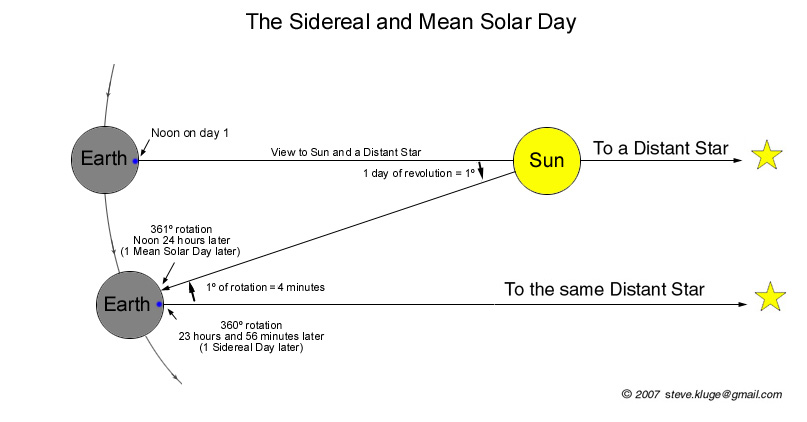
\includegraphics[width=1\linewidth]{sidereal_day.jpg}
   \caption{}
   \label{fig:Ng1} 
\end{subfigure}

\begin{subfigure}[b]{0.55\textwidth}
   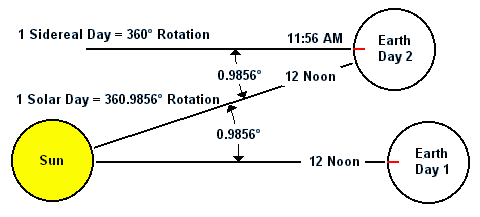
\includegraphics[width=1\linewidth]{sidereal_solar_day.png}
   \caption{}
   \label{fig:Ng2}
\end{subfigure}

\caption[Sidereal days]{(a) D'ia sideral respecto a una estrella lejana. Notar que esta estrella no se mueve, sino que es la Tierra la que aparentemente se mueve. Lo que implica que, gracias a la traslaci'on y rotaci'on, esta estrella saldr'a $\sim 4$ minutos antes que el d'ia anterior del horizonte. (b) Diferencia entre d'ia sideral y solar.} \label{dia_sideral}
\end{figure}

El d'ia sideral es el tiempo para que una estrella vuelva a alcanzar la misma posici'on en el cielo (23 horas con 56 minutos). Mientras que el d'ia solar es el tiempo de tr'ansito del Sol entre dos meridianos para alg'un lugar en particular (24 horas); por ejemplo, el tiempo que hay entre el mediod'ia y el mediod'ia del d'ia siguiente. De manera que se espera que una estrella logre alcanzar la misma posici'on que alcanz'o hoy, pero 4 minutos antes con respecto al d'ia anterior, como se ve en la Figura \ref{posicion_dia_sideral}.

\begin{figure}[!ht]
\begin{center}
\begin{tabular}{ll}
  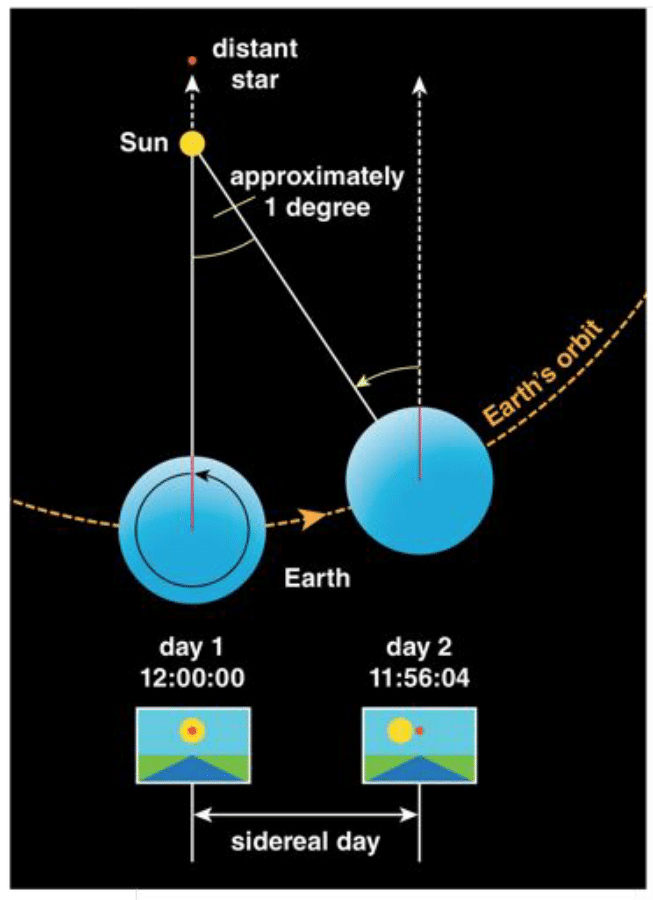
\includegraphics[width=0.35\textwidth]{sidereal_day_positions.png}
\end{tabular}
\caption{Variaci'on de una estrella a medida que va avanzando la Tierra en su 'orbita. Como se puede apreciar en la imagen, una estrella vuelve a alcanzar la misma posici'on en el cielo que alcanz'o el d'ia anterior 4 minutos antes.}\label{posicion_dia_sideral}
\end{center} 
\end{figure}

\vspace{3mm}

\textbf{Problema 4.} Chile y su horario. Santiago, junto con todo Chile, deber'ia tener el horario \texttt{GMT $-5$}. Sin embargo, el que se usa es el horario \texttt{GMT $-4$}. Basados en esto, ?`a qu'e hora, aproximadamente, el Sol alcanza su m'axima altura y por qu'e?

\emph{Soluci'on: }

La Figura \ref{GMT} muestra los horarios GMT (Greenwich Mean Time) que deber'ian tener los pa'ises s'olo en funci'on de sus meridianos geogr'aficos. En extricto rigor, estos horarios est'an pensados para que el Sol alcance su m'axima altura al mediod'ia. 

\begin{figure}[!ht]
\begin{center}
\begin{tabular}{ll}
  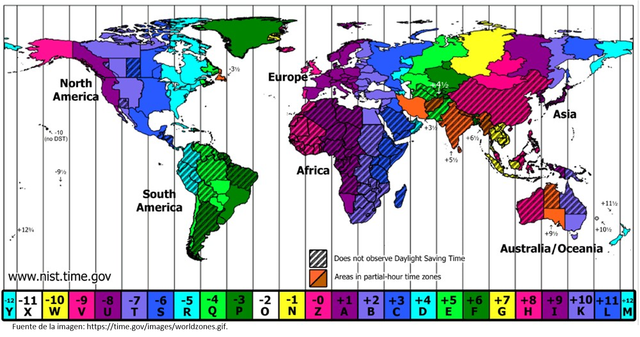
\includegraphics[width=0.58\textwidth]{gmt.png}
\end{tabular}
\caption{Horarios GMT seg'un la posici'on geogr'afica, basado principalmente en los meridianos.}\label{GMT}
\end{center} 
\end{figure}

Cada casilla en la Figura \ref{GMT} muestra un huso horario. Se toma referencia el meridiano 0 (Greenwich). Se a'nade 1 hora por cada huso horario que se recorra hacia el Este y se resta 1 hora hacia el Oeste.

Si se observa bien la Figura \ref{GMT}, Chile cae en la casilla \texttt{GMT $-5$}. Pero usamos el horario  \texttt{GMT $-4$}. En teor'ia, en el dibujo, el Sol va avanzando e iluminando de derecha a izquierda a medida que la Tierra rota. Ello quiere decir que adoptamos un horario en el que el mediod'ia pasa antes de lo que en realidad sucede. Por lo que, por ejemplo, cuando el Sol realmente alcanza su m'axima altura nosotros ya hab'iamos asumido que 'este lo hab'ia alcanzado una hora antes. As'i, en vez de ser mediod'ia, ser'an las 1 de la tarde. En el horario de verano asumimos un huso horario de \texttt{GMT $-3$} (cuando siempre deber'iamos asumir un \texttt{GMT $-5$}), por lo que en verano el Sol alcanzar'a su m'axima altura a las 2 de la tarde, aproximadamente; dado que ahora habr'a un desfase de 2 horas.

?`Por qu'e se realizan estos cambios de horario? Ello tiene que ver m'as que todo por una causa civil: mejor aprovechamiento de la luz natural. Es decir, se trata de ``optimizar'' lo m'aximo la luz natural y, por ejemplo, se logran abaratar costos asociados con energ'ia utilizada en iluminaci'on.
\end{document}